\documentclass[]{book}
\usepackage{lmodern}
\usepackage{amssymb,amsmath}
\usepackage{ifxetex,ifluatex}
\usepackage{fixltx2e} % provides \textsubscript
\ifnum 0\ifxetex 1\fi\ifluatex 1\fi=0 % if pdftex
  \usepackage[T1]{fontenc}
  \usepackage[utf8]{inputenc}
\else % if luatex or xelatex
  \ifxetex
    \usepackage{mathspec}
  \else
    \usepackage{fontspec}
  \fi
  \defaultfontfeatures{Ligatures=TeX,Scale=MatchLowercase}
\fi
% use upquote if available, for straight quotes in verbatim environments
\IfFileExists{upquote.sty}{\usepackage{upquote}}{}
% use microtype if available
\IfFileExists{microtype.sty}{%
\usepackage{microtype}
\UseMicrotypeSet[protrusion]{basicmath} % disable protrusion for tt fonts
}{}
\usepackage{hyperref}
\hypersetup{unicode=true,
            pdftitle={Microeconometrics - e-Notes: Practice guide using R},
            pdfauthor={Jaime MONTANA},
            pdfborder={0 0 0},
            breaklinks=true}
\urlstyle{same}  % don't use monospace font for urls
\usepackage{natbib}
\bibliographystyle{apalike}
\usepackage{color}
\usepackage{fancyvrb}
\newcommand{\VerbBar}{|}
\newcommand{\VERB}{\Verb[commandchars=\\\{\}]}
\DefineVerbatimEnvironment{Highlighting}{Verbatim}{commandchars=\\\{\}}
% Add ',fontsize=\small' for more characters per line
\usepackage{framed}
\definecolor{shadecolor}{RGB}{248,248,248}
\newenvironment{Shaded}{\begin{snugshade}}{\end{snugshade}}
\newcommand{\KeywordTok}[1]{\textcolor[rgb]{0.13,0.29,0.53}{\textbf{#1}}}
\newcommand{\DataTypeTok}[1]{\textcolor[rgb]{0.13,0.29,0.53}{#1}}
\newcommand{\DecValTok}[1]{\textcolor[rgb]{0.00,0.00,0.81}{#1}}
\newcommand{\BaseNTok}[1]{\textcolor[rgb]{0.00,0.00,0.81}{#1}}
\newcommand{\FloatTok}[1]{\textcolor[rgb]{0.00,0.00,0.81}{#1}}
\newcommand{\ConstantTok}[1]{\textcolor[rgb]{0.00,0.00,0.00}{#1}}
\newcommand{\CharTok}[1]{\textcolor[rgb]{0.31,0.60,0.02}{#1}}
\newcommand{\SpecialCharTok}[1]{\textcolor[rgb]{0.00,0.00,0.00}{#1}}
\newcommand{\StringTok}[1]{\textcolor[rgb]{0.31,0.60,0.02}{#1}}
\newcommand{\VerbatimStringTok}[1]{\textcolor[rgb]{0.31,0.60,0.02}{#1}}
\newcommand{\SpecialStringTok}[1]{\textcolor[rgb]{0.31,0.60,0.02}{#1}}
\newcommand{\ImportTok}[1]{#1}
\newcommand{\CommentTok}[1]{\textcolor[rgb]{0.56,0.35,0.01}{\textit{#1}}}
\newcommand{\DocumentationTok}[1]{\textcolor[rgb]{0.56,0.35,0.01}{\textbf{\textit{#1}}}}
\newcommand{\AnnotationTok}[1]{\textcolor[rgb]{0.56,0.35,0.01}{\textbf{\textit{#1}}}}
\newcommand{\CommentVarTok}[1]{\textcolor[rgb]{0.56,0.35,0.01}{\textbf{\textit{#1}}}}
\newcommand{\OtherTok}[1]{\textcolor[rgb]{0.56,0.35,0.01}{#1}}
\newcommand{\FunctionTok}[1]{\textcolor[rgb]{0.00,0.00,0.00}{#1}}
\newcommand{\VariableTok}[1]{\textcolor[rgb]{0.00,0.00,0.00}{#1}}
\newcommand{\ControlFlowTok}[1]{\textcolor[rgb]{0.13,0.29,0.53}{\textbf{#1}}}
\newcommand{\OperatorTok}[1]{\textcolor[rgb]{0.81,0.36,0.00}{\textbf{#1}}}
\newcommand{\BuiltInTok}[1]{#1}
\newcommand{\ExtensionTok}[1]{#1}
\newcommand{\PreprocessorTok}[1]{\textcolor[rgb]{0.56,0.35,0.01}{\textit{#1}}}
\newcommand{\AttributeTok}[1]{\textcolor[rgb]{0.77,0.63,0.00}{#1}}
\newcommand{\RegionMarkerTok}[1]{#1}
\newcommand{\InformationTok}[1]{\textcolor[rgb]{0.56,0.35,0.01}{\textbf{\textit{#1}}}}
\newcommand{\WarningTok}[1]{\textcolor[rgb]{0.56,0.35,0.01}{\textbf{\textit{#1}}}}
\newcommand{\AlertTok}[1]{\textcolor[rgb]{0.94,0.16,0.16}{#1}}
\newcommand{\ErrorTok}[1]{\textcolor[rgb]{0.64,0.00,0.00}{\textbf{#1}}}
\newcommand{\NormalTok}[1]{#1}
\usepackage{longtable,booktabs}
\usepackage{graphicx,grffile}
\makeatletter
\def\maxwidth{\ifdim\Gin@nat@width>\linewidth\linewidth\else\Gin@nat@width\fi}
\def\maxheight{\ifdim\Gin@nat@height>\textheight\textheight\else\Gin@nat@height\fi}
\makeatother
% Scale images if necessary, so that they will not overflow the page
% margins by default, and it is still possible to overwrite the defaults
% using explicit options in \includegraphics[width, height, ...]{}
\setkeys{Gin}{width=\maxwidth,height=\maxheight,keepaspectratio}
\IfFileExists{parskip.sty}{%
\usepackage{parskip}
}{% else
\setlength{\parindent}{0pt}
\setlength{\parskip}{6pt plus 2pt minus 1pt}
}
\setlength{\emergencystretch}{3em}  % prevent overfull lines
\providecommand{\tightlist}{%
  \setlength{\itemsep}{0pt}\setlength{\parskip}{0pt}}
\setcounter{secnumdepth}{5}
% Redefines (sub)paragraphs to behave more like sections
\ifx\paragraph\undefined\else
\let\oldparagraph\paragraph
\renewcommand{\paragraph}[1]{\oldparagraph{#1}\mbox{}}
\fi
\ifx\subparagraph\undefined\else
\let\oldsubparagraph\subparagraph
\renewcommand{\subparagraph}[1]{\oldsubparagraph{#1}\mbox{}}
\fi

%%% Use protect on footnotes to avoid problems with footnotes in titles
\let\rmarkdownfootnote\footnote%
\def\footnote{\protect\rmarkdownfootnote}

%%% Change title format to be more compact
\usepackage{titling}

% Create subtitle command for use in maketitle
\providecommand{\subtitle}[1]{
  \posttitle{
    \begin{center}\large#1\end{center}
    }
}

\setlength{\droptitle}{-2em}

  \title{Microeconometrics - e-Notes: Practice guide using R}
    \pretitle{\vspace{\droptitle}\centering\huge}
  \posttitle{\par}
    \author{Jaime MONTANA}
    \preauthor{\centering\large\emph}
  \postauthor{\par}
      \predate{\centering\large\emph}
  \postdate{\par}
    \date{Updated the 2019-09-21}

\usepackage{booktabs}

\begin{document}
\maketitle

{
\setcounter{tocdepth}{1}
\tableofcontents
}
\chapter{Introduction}\label{introduction}

\begin{center}
\includegraphics[width=0.9\linewidth]{./images/1200px-Logo_pse_petit} \end{center}

\section{General Info}\label{general-info}

\subsection{Contact information}\label{contact-information}

\begin{itemize}
\tightlist
\item
  \textbf{Webpage:}
\item
  \textbf{E-mail:}
  \href{mailto:jaimem.montana@gmail.com}{\nolinkurl{jaimem.montana@gmail.com}}
\item
  \textbf{Slack:} I will send you the link.
\end{itemize}

Feel free to email at any time to ask questions about the methods
covered in class, although I will prioritize communications over the
Slack channel. In this way everyone can benefit from others' questions
and answers. If anyone knows how to solve a problem, debug or fix the
code in the Slack forum s/he can help.

There are some rules for making questions on the procedures. Before
asking, it is \textbf{mandatory} that you consult the documentation of
the function/package; also try to search the answer in a public forum
(i.e.~Stack Overflow). If after that you still have troubles, post the
question taking the following into consideration:

\begin{itemize}
\tightlist
\item
  Be clear and concise, so everyone can understand you
\item
  Be as specific as possible, being clear and straightforward
\item
  Include sufficient information: your goal, the code, the data,
  everething in order to reproduce the error
\end{itemize}

Also, you can ask questions about the interpretation of the results, the
theory behind, and the like.

\section{Objective}\label{objective}

This class notes are an interactive e-material for the Microeconometrics
course in the master APE in Paris School of Economics. The aim of this
notes is to provide an e-learning material to apply the theorical
concepts of the class. The notes are in \textbf{open review}: comments,
corrections or contributions that you can make to this part of the
course and the material provided are more than welcome.

This part of the course does not cover the theory, and assumes you
already had it covered and understood. We will depart from the theory
with direct application of the methods.

\section{Prerequisites}\label{prerequisites}

Please install R and Rstudio in your laptop. Here is a video to install
R and Rstudio in windows and mac. If you have questions or you could not
manage to install it, bring your laptop next session. I will help out
for the installation.

\begin{itemize}
\tightlist
\item
  windows-os: \href{https://www.youtube.com/watch?v=9-RrkJQQYqY}{For
  Windows click this link}
\item
  mac-os: \href{https://www.youtube.com/watch?v=GLLZhc_5enQ}{For Mac-OS
  click this link}
\end{itemize}

Why \textbf{R}? R is a \textbf{free} software programming language and a
software environment for statistical computing and graphics. The R
language is widely used among statisticians, economist, in finance and
academics circles.

\begin{itemize}
\item
  R is a \textbf{free} software, easy to install and runs in multiple
  OS.
\item
  A lot of documentation and forums. Excellent documentation on
  packages.
\item
  Very active community which allow to use other people codes and
  projects.
\item
  \textbf{Great} visualization tools thanks to \emph{ggplot} and
  \emph{plotly} packages.
\item
  If you understand the logic behind R you will get into every
  statistical software very easily.
\item
  Everything seems hard at the beginning. Just try and ask.
\end{itemize}

\textbf{A prior knowledge on the use of R is required.} We don`t have
much time to cover the basics. For an introduction to R you can check
the following material:

\begin{itemize}
\tightlist
\item
  \href{https://www.econometrics-with-r.org/1-1-a-very-short-introduction-to-r-and-rstudio.html}{Introduction
  to Econometrics with R, Chapter 1 - 6, by Christoph Hanck et al.}
\item
  \href{https://scpoecon.github.io/ScPoEconometrics/R-intro.html}{Introduction
  to Econometrics with R by Florian Oswald, Jean-Marc Robin and Vincent
  Viers}
\end{itemize}

\section{Course structure}\label{course-structure}

\begin{itemize}
\item
  We will have only 3 sessions (2 hours each)
\item
  Bring your laptop with R installed on it
\item
  The material for each session will be online just before each session.
  In that way you can follow from the e-notes and do the exercises with
  me during class
\item
  What to expect from each session:

\begin{verbatim}
1. Brief explanation on the method (how it works)
2. Replication of a published paper that applies the method (downloading data, cleaning data, estimation, tables and plotting results)
3. Discussion on the interpretation of the results
4. Q/A
\end{verbatim}
\item
  There will be \emph{suggested exercises}. These are \textbf{not
  mandatory}, but remember that if you want to master something, you
  need to practice. I will be happy to give some feedback on the
  suggested exercises if you want.
\end{itemize}

\chapter{Session I - Quantile
regression}\label{session-i---quantile-regression}

\begin{center}
\includegraphics[width=0.9\linewidth]{./images/1200px-Logo_pse_petit} \end{center}

\section{Objective}\label{objective-1}

This first class is to introduce your to using R for implementing
quantile regressions. Therefore, we are going to:

\begin{enumerate}
\def\labelenumi{\arabic{enumi}.}
\item
  Understand the mathematical procedure behind the QR estmation and its
  computation (both for the estimates and for the the standard errors).
  This will help understanding the interpretation of the results
  obtained when applying the procedure in other contexts.
\item
  Reproduce a paper's tables and results using quantile regression

\begin{verbatim}
a) Import the data
b) Clean the data
c) Reproduce the summary statistics table
d) reproduce the regressions tables
\end{verbatim}
\item
  Interpret the results
\item
  Ways to communicate the results (plotting in R)
\end{enumerate}

In the last part of the lecture I will just mention and make reference
to other classes of QR estimators so you can investigate more on them;

\section{Quantile Regression}\label{quantile-regression}

\textbf{For a summary on what is the intuition and objective of quantile
regression check the article ``Quantile Regression''
\citep{koenker2001quantile}.}

QR is a method that allows you to analyse the relation between \(x\) and
\(y\) across the \(y\) distribution. It is useful when the researcher
thinks there are \emph{heterogeneous effects} at different values of the
indipendent variable. It is important to remark that the heterogeneity
is on the \textbf{outcome} \(y\). Also, it is widely used in presence of
outliers and extreme events (infinite variance), for OLS is inconsistent
in such cases while the median is always defined and consistent. For
quantiles other than \(\tau = 0.5\) the estimation is robust, too.

From the class we know the relationship between the \textbf{definition
of the estimator}, the \textbf{risk function} used in the optimization
(in the case of the lector the \emph{`LAD function'}, when
\(\tau = 0.5\)) and that we need to solve numerically the
\textbf{optimization program} in order to identify the parameters of
interest. Accordingly, we will explain how the algorithm works and we
are going to perform the numerical optimization by hand from the
simplest case to more complex problems.

\subsection{Geometric interpretation}\label{geometric-interpretation}

From \citep{koenker2001quantile}:

\begin{quote}
Quantiles seem inseparably linked to the operations of ordering and
sorting the sample observations that are usually used to define them. So
it comes as a mild surprise to observe that we can define \textbf{the
quantiles} through a simple alternative expedient \textbf{as an
optimization problem}. Just as we can define the sample mean as the
solution to the problem of minimizing a sum of squared residuals, we can
define the \emph{median as the solution to the problem of minimizing a
sum of absolute residuals}. The symmetry of the piecewise linear
absolute value function implies that the minimization of the sum of
absolute residuals must equate the number of positive and negative
residuals, thus assuring that there are the same number of observations
above and below the median. What about the other quantiles? Since the
symmetry of the absolute value yields the median, perhaps minimizing a
sum of asymmetrically weighted absolute residuals---simply giving
differing weights to positive and negative residuals---would yield the
quantiles. This is indeed the case.
\end{quote}

The slope of the coefficient is dividing the error space in two parts
according to the desired proportion. It is important to notice that we
are considering the error space, we are referring to the conditioning
quantile. The difference with the OLS is then clear since the two
processes are not comparable. While OLS might provide causal linkages,
this is prevented in QR precisely for this reason.

Let's generate some data to see how the line bisects the error space.
Since we are generating random data the first thing is to set a seed so
our example is reproducible. Then, we generate variance for our error
term (not constant) and set an intercept and define the slope. We set
everything in a `data.frame' objecto to plot it using the package
`ggplot2'\citep{R-ggplot2}.

\begin{Shaded}
\begin{Highlighting}[]
\KeywordTok{set.seed}\NormalTok{(}\DecValTok{464}\NormalTok{)}
\NormalTok{npoints <-}\StringTok{ }\DecValTok{150}
\NormalTok{x <-}\StringTok{ }\KeywordTok{seq}\NormalTok{(}\DecValTok{0}\NormalTok{,}\DecValTok{10}\NormalTok{,}\DataTypeTok{length.out =}\NormalTok{ npoints)        }
\NormalTok{sigma <-}\StringTok{ }\FloatTok{0.1} \OperatorTok{+}\StringTok{ }\FloatTok{0.25}\OperatorTok{*}\KeywordTok{sqrt}\NormalTok{(x) }\OperatorTok{+}\StringTok{ }\KeywordTok{ifelse}\NormalTok{(x}\OperatorTok{>}\DecValTok{6}\NormalTok{,}\DecValTok{1}\NormalTok{,}\DecValTok{0}\NormalTok{)                    }
\NormalTok{intercept <-}\StringTok{ }\DecValTok{2}                                
\NormalTok{slope <-}\StringTok{ }\FloatTok{0.2}                              
                             
\NormalTok{error <-}\StringTok{ }\KeywordTok{rnorm}\NormalTok{(npoints,}\DataTypeTok{mean =} \DecValTok{0}\NormalTok{, }\DataTypeTok{sd =}\NormalTok{ sigma)      }
\NormalTok{y <-}\StringTok{ }\NormalTok{intercept }\OperatorTok{+}\StringTok{ }\NormalTok{slope}\OperatorTok{*}\NormalTok{x }\OperatorTok{+}\StringTok{ }\NormalTok{error                    }
\NormalTok{dat <-}\StringTok{ }\KeywordTok{data.frame}\NormalTok{(x,y)}
\end{Highlighting}
\end{Shaded}

Let's plot our synthetic data. We are going to plot the line crossing
the 90th percentile conditioning on \(X\) (dashed red line), the OLS
curve (blue line with confidence intervals in grey) and the LAD
regression (regression to the median, \(\tau = 0.5\))

\begin{Shaded}
\begin{Highlighting}[]
\KeywordTok{ggplot}\NormalTok{(dat, }\KeywordTok{aes}\NormalTok{(x,y)) }\OperatorTok{+}\StringTok{ }\KeywordTok{geom_point}\NormalTok{() }\OperatorTok{+}\StringTok{ }\KeywordTok{geom_smooth}\NormalTok{(}\DataTypeTok{method=}\StringTok{"lm"}\NormalTok{) }\OperatorTok{+}\StringTok{ }
\StringTok{        }\KeywordTok{geom_quantile}\NormalTok{(}\DataTypeTok{quantiles =} \FloatTok{0.9}\NormalTok{, }\DataTypeTok{colour =} \StringTok{'red'}\NormalTok{, }\DataTypeTok{linetype=}\StringTok{"dotted"}\NormalTok{) }\OperatorTok{+}
\StringTok{        }\KeywordTok{geom_quantile}\NormalTok{(}\DataTypeTok{quantiles =} \FloatTok{0.5}\NormalTok{, }\DataTypeTok{colour =} \StringTok{'green'}\NormalTok{) }
\end{Highlighting}
\end{Shaded}

\begin{verbatim}
## Smoothing formula not specified. Using: y ~ x
## Smoothing formula not specified. Using: y ~ x
\end{verbatim}

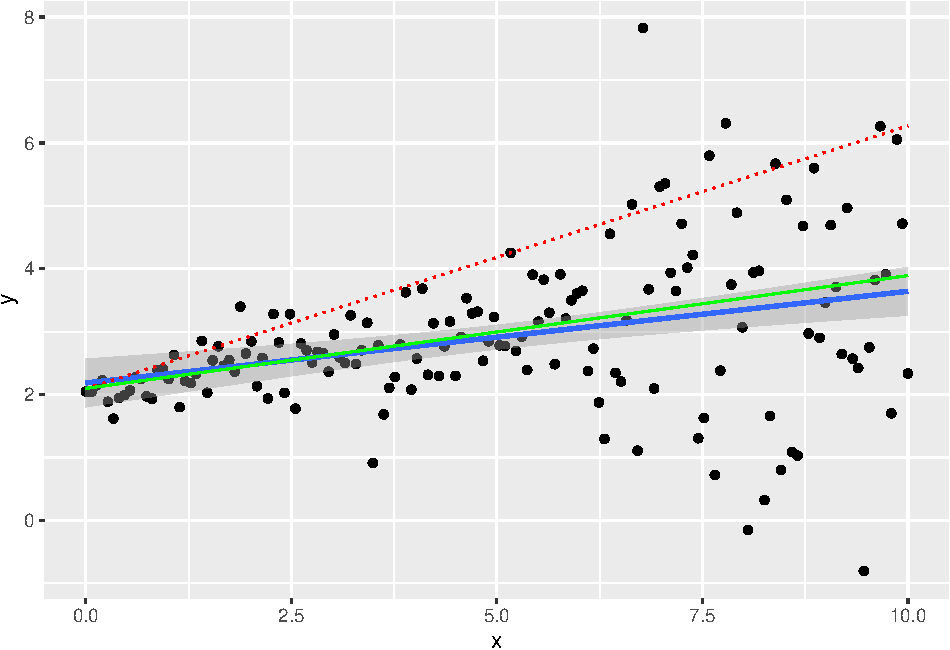
\includegraphics{Material_files/figure-latex/unnamed-chunk-3-1.pdf}

We can interpret the causal relationship in quantile regression only
under rank invariant condition. This requires that individuals have
always the same ranking in the distribution of \(Y(X)\) no matter the
\(X\). This is difficult to verify or believe in actual applications,
but feasible in theory.

Under the rank invariant condition \(\beta_{\tau}\) can be interpreted
as the effect on \(Y\) of an increase of one unit of \(X\) among
entities at rank \(\tau\) in the distribution \(Y|X=x\).

\subsection{Estimation of the
quantiles}\label{estimation-of-the-quantiles}

In order to understand how the estimation procedure works first we are
going to set up the most simple problem, we are going to solve to find
the value for a specific quantile in a distribution.

\begin{Shaded}
\begin{Highlighting}[]
\NormalTok{n =}\StringTok{ }\DecValTok{101}
\KeywordTok{set.seed}\NormalTok{(}\DecValTok{10}\NormalTok{)}
\NormalTok{y =}\StringTok{ }\KeywordTok{rlnorm}\NormalTok{(n)}
\KeywordTok{quantile}\NormalTok{(y, }\FloatTok{0.3}\NormalTok{)}
\end{Highlighting}
\end{Shaded}

\begin{verbatim}
##       30% 
## 0.5092247
\end{verbatim}

\begin{Shaded}
\begin{Highlighting}[]
\KeywordTok{library}\NormalTok{(lpSolve)}
\NormalTok{tau =}\StringTok{ }\FloatTok{0.3}
\NormalTok{A1 =}\StringTok{ }\KeywordTok{cbind}\NormalTok{(}\KeywordTok{diag}\NormalTok{(}\DecValTok{2}\OperatorTok{*}\NormalTok{n),}\DecValTok{0}\NormalTok{)}
\NormalTok{A2 =}\StringTok{ }\KeywordTok{cbind}\NormalTok{(}\KeywordTok{diag}\NormalTok{(n) , }\OperatorTok{-}\KeywordTok{diag}\NormalTok{( n) , }\DecValTok{1}\NormalTok{)}
\NormalTok{r =}\StringTok{ }\KeywordTok{lp}\NormalTok{(}\StringTok{"min"}\NormalTok{, }
       \KeywordTok{c}\NormalTok{(}\KeywordTok{rep}\NormalTok{(tau ,n),}\KeywordTok{rep}\NormalTok{(}\DecValTok{1} \OperatorTok{-}\StringTok{ }\NormalTok{tau,n),}\DecValTok{0}\NormalTok{),}
       \KeywordTok{rbind}\NormalTok{(A1, A2),}
       \KeywordTok{c}\NormalTok{(}\KeywordTok{rep}\NormalTok{(}\StringTok{">="}\NormalTok{, }\DecValTok{2}\OperatorTok{*}\NormalTok{n) , }\KeywordTok{rep}\NormalTok{(}\StringTok{"="}\NormalTok{, n)),}
       \KeywordTok{c}\NormalTok{(}\KeywordTok{rep}\NormalTok{(}\DecValTok{0}\NormalTok{ ,}\DecValTok{2}\OperatorTok{*}\NormalTok{n), y))}
\NormalTok{r}
\end{Highlighting}
\end{Shaded}

\begin{verbatim}
## Success: the objective function is 30.98553
\end{verbatim}

\subsection{Estimation of the quantile
regression}\label{estimation-of-the-quantile-regression}

\subsubsection{The One variable case}\label{the-one-variable-case}

\subsubsection{The multiple regressor
case}\label{the-multiple-regressor-case}

\section{Replication of a paper using quantile
regression}\label{replication-of-a-paper-using-quantile-regression}

We are going to replicate the quantile regression procedure by
\citep{abrevaya2002effects}. In the
\href{https://link.springer.com/article/10.1007/s001810000052}{paper}
the author investigates the impact of different demographic
characteristics and maternal behaviour on the weight at birth in the
United States in 1992 and 1996. Why is this relevant:

\begin{itemize}
\tightlist
\item
  There is a correlation between health problems after birth for
  underweight chidren
\item
  There might be a relation with labor market participation and
  educational attaintment later in life
\item
  There are incentives to create specific programs to deal with
  underweight children; it is important to understand such behaviours
\end{itemize}

\subsubsection{Data:}\label{data}

In order to get the data we access the following
\href{https://www.nber.org/data/vital-statistics-natality-data.html}{link}.
Here you can download the `NCHS' Vital Statistics Natality Birth Data',
which is the data used in the paper. We are using only the 1992 and 1996
waves. To download the data follow this link
\href{https://www.nber.org/natality/1992/natl1992.csv.zip}{for the zip
CSV file of 1992}. One important thing to do when analizing the data is
understand your data before the actual analysis. Before you start you
take a minute or two to consider:

\begin{itemize}
\tightlist
\item
  What is the data?
\item
  Where does it come from? What is the universe, the population and what
  is your sample.
\item
  What is the shape, format of your data? Do I have access to a data
  dictionary?
\end{itemize}

In this case many of this questions are available in the documentation
that is provided {[}at the following link{]}
(\url{https://www.nber.org/natality/1992/natl1992.pdf}) detailing every
variable in the dataset. From the documentation we can see the kind of
information (a glimpse of the amount of variables) and the data counts
(\(4'069'428\) observations). An indicator of the size of the data is
the size of the file: the zip file is \emph{156 Mb} and the uncompressed
version of the CSV \emph{2.07 GB}! Even if this does not seem much,
consider that all this data is stored in the cache of your RAM memory,
and it can easily slow down even recent machines. For this reason it is
better to read in only the columns that we are interested in. This
requires reading the manual and a prior inspection of a subset of the
data, which allows you to know the structure, column types and other
properties. The most efficient function to open plain text files is
\emph{`fread'} from the \emph{`data.table'} package
\citep{R-data.table}. First let's investigate the data. The first thing
to do is to load the required libraries int the current session:

\begin{itemize}
\tightlist
\item
  \emph{`data.table'} to open the data
\item
  \emph{`quantreg'} to perform the quantile regression estimation
\item
  \emph{`stargazer'} to export the results in latex
\item
  \emph{`dplyr'} to manipulate the data to create the summary statistics
\end{itemize}

\begin{Shaded}
\begin{Highlighting}[]
\KeywordTok{library}\NormalTok{(data.table)}
\KeywordTok{library}\NormalTok{(quantreg)}
\KeywordTok{library}\NormalTok{(stargazer)}
\KeywordTok{library}\NormalTok{(dplyr)}
\KeywordTok{library}\NormalTok{(kableExtra)}
\end{Highlighting}
\end{Shaded}

\begin{Shaded}
\begin{Highlighting}[]
\NormalTok{path_source <-}\StringTok{ "YOUR PATH GOES HERE"}
\CommentTok{# for macOS and linux: use / in your path to data}
\CommentTok{# for Win: rembember to use \textbackslash{}\textbackslash{} instead of /}
\end{Highlighting}
\end{Shaded}

\begin{Shaded}
\begin{Highlighting}[]
\NormalTok{data <-}\StringTok{ }\KeywordTok{fread}\NormalTok{(path_source, }\DataTypeTok{nrows =} \KeywordTok{c}\NormalTok{(}\DecValTok{100}\NormalTok{))}
\KeywordTok{head}\NormalTok{(data[,}\KeywordTok{c}\NormalTok{(}\DecValTok{35}\OperatorTok{:}\DecValTok{41}\NormalTok{)])}
\end{Highlighting}
\end{Shaded}

\begin{verbatim}
##    mage12 mage8 ormoth orracem mraceimp mrace mrace3
## 1:      9     4      0       7       NA     2      3
## 2:      9     4      0       7       NA     2      3
## 3:      8     3      0       7       NA     2      3
## 4:      8     3      0       6       NA     1      1
## 5:      5     2      0       6       NA     1      1
## 6:      9     4      0       6       NA     1      1
\end{verbatim}

\begin{Shaded}
\begin{Highlighting}[]
\NormalTok{type_of_data <-}\StringTok{ }\NormalTok{data }\OperatorTok\StringTok{ }\KeywordTok{summarise_all}\NormalTok{(typeof)}
\NormalTok{type_of_data[}\DecValTok{35}\OperatorTok{:}\DecValTok{41}\NormalTok{]}
\end{Highlighting}
\end{Shaded}

\begin{verbatim}
##    mage12   mage8  ormoth orracem mraceimp   mrace  mrace3
## 1 integer integer integer integer  logical integer integer
\end{verbatim}

Now that we have had a look at the content of the database, let's import
the data and clean it. To import only the relevant variables of the
paper we create a list containing all the relevant variables for the
estimation. I used the codebook to construct this list. Then we use this
list within `fread()' to import solely the desired columns.

\begin{Shaded}
\begin{Highlighting}[]
\NormalTok{desired <-}\StringTok{ }\KeywordTok{c}\NormalTok{(}\StringTok{"birmon"}\NormalTok{,}\StringTok{"mrace3"}\NormalTok{,}\StringTok{"dmage"}\NormalTok{,}\StringTok{"dbirwt"}\NormalTok{,}\StringTok{"dplural"}\NormalTok{,}\StringTok{"stnatexp"}\NormalTok{,}
             \StringTok{"mraceimp"}\NormalTok{,}\StringTok{"dmarimp"}\NormalTok{,}\StringTok{"mageimp"}\NormalTok{,}\StringTok{"cseximp"}\NormalTok{,}\StringTok{"dmar"}\NormalTok{,}\StringTok{"meduc6"}\NormalTok{, }
             \StringTok{"wtgain"}\NormalTok{, }\StringTok{"mpre5"}\NormalTok{, }\StringTok{"tobacco"}\NormalTok{,}\StringTok{"cigar"}\NormalTok{, }\StringTok{"csex"}\NormalTok{, }\StringTok{"plurimp"}\NormalTok{, }\StringTok{"restatus"}\NormalTok{)}

\NormalTok{data <-}\StringTok{ }\KeywordTok{fread}\NormalTok{(path_source, }\DataTypeTok{select =}\NormalTok{ desired)}
\end{Highlighting}
\end{Shaded}

Following the indications of the paper:

\begin{quote}
To cut down he sample size, we have decided to use only births occurring
in June {[}\ldots{}{]} There is no evidence that suggest that the June
samplediffers in any meaningful way to the full sample. The sample was
further limited to singleton births and mothers who were either white or
black, between ages 18 and 45, and residents of the United States.
Observations for which there was missing information on any relevant
variable were also dropped. Unfortunately, all births occurring in
California, Indiana, New York, and South Dakota had to be dropped from
the sample since these states either did not asked a question about
smoking during pregnancy or did not ask it in a form compatible with
NHCS standards\ldots{}
\end{quote}

We need to apply the following filters:

\begin{itemize}
\tightlist
\item
  Remove all obs. in months different than the sixth (June)
\item
  Remove all non white or non black mothers
\item
  Remove all obs. which age is not in {[}18,45{]} group
\item
  Remove the non stated weights
\item
  Remove all the obs. from California, New York, Indiana and South
  Dakota
\end{itemize}

\begin{Shaded}
\begin{Highlighting}[]
\NormalTok{data <-}\StringTok{ }\NormalTok{data[}\KeywordTok{which}\NormalTok{(data}\OperatorTok{$}\NormalTok{restatus}\OperatorTok{!=}\DecValTok{4}\NormalTok{),]}
\NormalTok{data <-}\StringTok{ }\NormalTok{data[}\KeywordTok{which}\NormalTok{(data}\OperatorTok{$}\NormalTok{birmon}\OperatorTok{==}\DecValTok{6}\NormalTok{),]}
\NormalTok{data <-}\StringTok{ }\NormalTok{data[}\KeywordTok{which}\NormalTok{(data}\OperatorTok{$}\NormalTok{mrace3}\OperatorTok{!=}\DecValTok{2}\NormalTok{),]}
\NormalTok{data <-}\StringTok{ }\NormalTok{data[}\KeywordTok{which}\NormalTok{(data}\OperatorTok{$}\NormalTok{dmage}\OperatorTok{>}\DecValTok{17}\NormalTok{),]}
\NormalTok{data <-}\StringTok{ }\NormalTok{data[}\KeywordTok{which}\NormalTok{(data}\OperatorTok{$}\NormalTok{dmage}\OperatorTok{<}\DecValTok{46}\NormalTok{),]}
\NormalTok{data <-}\StringTok{ }\NormalTok{data[}\KeywordTok{which}\NormalTok{(data}\OperatorTok{$}\NormalTok{dbirwt}\OperatorTok{!=}\DecValTok{9999}\NormalTok{),]}
\NormalTok{data <-}\StringTok{ }\NormalTok{data[}\KeywordTok{which}\NormalTok{(data}\OperatorTok{$}\NormalTok{dplural}\OperatorTok{==}\DecValTok{1}\NormalTok{),]}
\NormalTok{data <-}\StringTok{ }\NormalTok{data[}\KeywordTok{which}\NormalTok{(}\OperatorTok{!}\NormalTok{(data}\OperatorTok{$}\NormalTok{stnatexp }\OperatorTok\StringTok{ }\KeywordTok{c}\NormalTok{(}\StringTok{"05"}\NormalTok{,}\StringTok{"33"}\NormalTok{,}\StringTok{"34"}\NormalTok{,}\StringTok{"15"}\NormalTok{,}\StringTok{"43"}\NormalTok{))),]}
\end{Highlighting}
\end{Shaded}

Moreover, we remove the missing observations. One particularity of many
of the variables of the database is that the missing values are coded,
meaning that are not representes by
\texttt{\textquotesingle{}NA\textquotesingle{}} but by a code that
changes in each variable. We are going to remove also the missing from
those variables:

\begin{Shaded}
\begin{Highlighting}[]
\NormalTok{data <-}\StringTok{ }\NormalTok{data[}\KeywordTok{which}\NormalTok{(}\OperatorTok{!}\NormalTok{(data}\OperatorTok{$}\NormalTok{plurimp }\OperatorTok\StringTok{ }\KeywordTok{c}\NormalTok{(}\DecValTok{1}\NormalTok{))),]}
\NormalTok{data <-}\StringTok{ }\NormalTok{data[}\KeywordTok{which}\NormalTok{(}\OperatorTok{!}\NormalTok{(data}\OperatorTok{$}\NormalTok{mraceimp }\OperatorTok\StringTok{ }\KeywordTok{c}\NormalTok{(}\DecValTok{1}\NormalTok{))),]}
\NormalTok{data <-}\StringTok{ }\NormalTok{data[}\KeywordTok{which}\NormalTok{(}\OperatorTok{!}\NormalTok{(data}\OperatorTok{$}\NormalTok{dmarimp }\OperatorTok\StringTok{ }\KeywordTok{c}\NormalTok{(}\DecValTok{1}\NormalTok{))),]}
\NormalTok{data <-}\StringTok{ }\NormalTok{data[}\KeywordTok{which}\NormalTok{(}\OperatorTok{!}\NormalTok{(data}\OperatorTok{$}\NormalTok{mageimp }\OperatorTok\StringTok{ }\KeywordTok{c}\NormalTok{(}\DecValTok{1}\NormalTok{))),]}
\NormalTok{data <-}\StringTok{ }\NormalTok{data[}\KeywordTok{which}\NormalTok{(}\OperatorTok{!}\NormalTok{(data}\OperatorTok{$}\NormalTok{cseximp }\OperatorTok\StringTok{ }\KeywordTok{c}\NormalTok{(}\DecValTok{1}\NormalTok{))),]}
\NormalTok{toKeep <-}\StringTok{ }\KeywordTok{c}\NormalTok{(}\StringTok{"dbirwt"}\NormalTok{, }\StringTok{"mrace3"}\NormalTok{,}\StringTok{"dmar"}\NormalTok{,}\StringTok{"dmage"}\NormalTok{,}\StringTok{"meduc6"}\NormalTok{, }\StringTok{"wtgain"}\NormalTok{, }\StringTok{"mpre5"}\NormalTok{, }\StringTok{"tobacco"}\NormalTok{,}\StringTok{"cigar"}\NormalTok{, }\StringTok{"csex"}\NormalTok{)}
\NormalTok{data <-}\StringTok{ }\KeywordTok{as.data.frame}\NormalTok{(data)}
\NormalTok{data <-}\StringTok{ }\NormalTok{data[,toKeep]}
\NormalTok{data <-}\StringTok{ }\NormalTok{data[}\KeywordTok{which}\NormalTok{(data}\OperatorTok{$}\NormalTok{dbirwt}\OperatorTok{!=}\DecValTok{9999}\NormalTok{),]}
\NormalTok{data <-}\StringTok{ }\NormalTok{data[}\KeywordTok{which}\NormalTok{(data}\OperatorTok{$}\NormalTok{wtgain}\OperatorTok{!=}\DecValTok{99}\NormalTok{),]}
\NormalTok{data <-}\StringTok{ }\NormalTok{data[}\KeywordTok{which}\NormalTok{(data}\OperatorTok{$}\NormalTok{dmage}\OperatorTok{!=}\DecValTok{99}\NormalTok{),]}
\NormalTok{data <-}\StringTok{ }\NormalTok{data[}\KeywordTok{which}\NormalTok{(data}\OperatorTok{$}\NormalTok{meduc6}\OperatorTok{!=}\DecValTok{6}\NormalTok{),]}
\NormalTok{data <-}\StringTok{ }\NormalTok{data[}\KeywordTok{which}\NormalTok{(data}\OperatorTok{$}\NormalTok{mpre5}\OperatorTok{!=}\DecValTok{5}\NormalTok{),]}
\NormalTok{data <-}\StringTok{ }\NormalTok{data[}\KeywordTok{which}\NormalTok{(data}\OperatorTok{$}\NormalTok{tobacco}\OperatorTok{!=}\DecValTok{9}\NormalTok{),]}
\NormalTok{data <-}\StringTok{ }\NormalTok{data[}\KeywordTok{which}\NormalTok{(data}\OperatorTok{$}\NormalTok{cigar}\OperatorTok{!=}\DecValTok{99}\NormalTok{),]}
\NormalTok{data <-}\StringTok{ }\NormalTok{data[}\KeywordTok{which}\NormalTok{(data}\OperatorTok{$}\NormalTok{wtgain }\OperatorTok{!=}\DecValTok{99}\NormalTok{),]}
\end{Highlighting}
\end{Shaded}

For the categorical variables (i.e.~education of the mother), we create
dummy variables. We keep the contrast (levels of reference) according to
the paper. In this way we will be able to compare the results.

\begin{Shaded}
\begin{Highlighting}[]
\NormalTok{data}\OperatorTok{$}\NormalTok{black <-}\StringTok{ }\KeywordTok{ifelse}\NormalTok{(data}\OperatorTok{$}\NormalTok{mrace3}\OperatorTok{==}\DecValTok{3}\NormalTok{,}\DecValTok{1}\NormalTok{,}\DecValTok{0}\NormalTok{)}
\NormalTok{data}\OperatorTok{$}\NormalTok{married <-}\StringTok{ }\KeywordTok{ifelse}\NormalTok{(data}\OperatorTok{$}\NormalTok{dmar}\OperatorTok{==}\DecValTok{1}\NormalTok{,}\DecValTok{1}\NormalTok{,}\DecValTok{0}\NormalTok{)}
\NormalTok{data}\OperatorTok{$}\NormalTok{agesq <-}\StringTok{ }\NormalTok{(data}\OperatorTok{$}\NormalTok{dmage)}\OperatorTok{^}\DecValTok{2}
\NormalTok{data}\OperatorTok{$}\NormalTok{hsgrad <-}\StringTok{ }\KeywordTok{ifelse}\NormalTok{(data}\OperatorTok{$}\NormalTok{meduc6}\OperatorTok{==}\DecValTok{3}\NormalTok{,}\DecValTok{1}\NormalTok{,}\DecValTok{0}\NormalTok{)}
\NormalTok{data}\OperatorTok{$}\NormalTok{somecoll <-}\StringTok{ }\KeywordTok{ifelse}\NormalTok{(data}\OperatorTok{$}\NormalTok{meduc6}\OperatorTok{==}\DecValTok{4}\NormalTok{,}\DecValTok{1}\NormalTok{,}\DecValTok{0}\NormalTok{)}
\NormalTok{data}\OperatorTok{$}\NormalTok{collgrad <-}\StringTok{ }\KeywordTok{ifelse}\NormalTok{(data}\OperatorTok{$}\NormalTok{meduc6}\OperatorTok{==}\DecValTok{5}\NormalTok{,}\DecValTok{1}\NormalTok{,}\DecValTok{0}\NormalTok{)}
\NormalTok{data}\OperatorTok{$}\NormalTok{natal2 <-}\StringTok{ }\KeywordTok{ifelse}\NormalTok{(data}\OperatorTok{$}\NormalTok{mpre5}\OperatorTok{==}\DecValTok{2}\NormalTok{,}\DecValTok{1}\NormalTok{,}\DecValTok{0}\NormalTok{)}
\NormalTok{data}\OperatorTok{$}\NormalTok{natal3 <-}\StringTok{ }\KeywordTok{ifelse}\NormalTok{(data}\OperatorTok{$}\NormalTok{mpre5}\OperatorTok{==}\DecValTok{3}\NormalTok{,}\DecValTok{1}\NormalTok{,}\DecValTok{0}\NormalTok{)}
\NormalTok{data}\OperatorTok{$}\NormalTok{novisit <-}\StringTok{ }\KeywordTok{ifelse}\NormalTok{(data}\OperatorTok{$}\NormalTok{mpre5}\OperatorTok{==}\DecValTok{4}\NormalTok{,}\DecValTok{1}\NormalTok{,}\DecValTok{0}\NormalTok{)}
\NormalTok{data}\OperatorTok{$}\NormalTok{nosmoke <-}\StringTok{ }\KeywordTok{ifelse}\NormalTok{(data}\OperatorTok{$}\NormalTok{tobacco}\OperatorTok{==}\DecValTok{2}\NormalTok{,}\DecValTok{1}\NormalTok{,}\DecValTok{0}\NormalTok{)}
\NormalTok{data}\OperatorTok{$}\NormalTok{boy <-}\StringTok{ }\KeywordTok{ifelse}\NormalTok{(data}\OperatorTok{$}\NormalTok{csex}\OperatorTok{==}\DecValTok{1}\NormalTok{,}\DecValTok{1}\NormalTok{,}\DecValTok{0}\NormalTok{)}
\end{Highlighting}
\end{Shaded}

We also relabel variables to match those in the paper:

\begin{Shaded}
\begin{Highlighting}[]
\NormalTok{finalVars <-}\StringTok{ }\KeywordTok{c}\NormalTok{(}\StringTok{"dbirwt"}\NormalTok{,}\StringTok{"black"}\NormalTok{, }\StringTok{"married"}\NormalTok{, }\StringTok{"dmage"}\NormalTok{, }\StringTok{"agesq"}\NormalTok{, }\StringTok{"hsgrad"}\NormalTok{, }\StringTok{"somecoll"}\NormalTok{, }\StringTok{"collgrad"}\NormalTok{, }\StringTok{"wtgain"}\NormalTok{, }\StringTok{"natal2"}\NormalTok{, }\StringTok{"natal3"}\NormalTok{, }\StringTok{"novisit"}\NormalTok{, }\StringTok{"nosmoke"}\NormalTok{, }\StringTok{"cigar"}\NormalTok{, }\StringTok{"boy"}\NormalTok{)}
\NormalTok{data <-}\StringTok{ }\NormalTok{data[, finalVars]}
\KeywordTok{names}\NormalTok{(data) <-}\StringTok{ }\KeywordTok{c}\NormalTok{(}\StringTok{"birwt"}\NormalTok{,}\StringTok{"black"}\NormalTok{, }\StringTok{"married"}\NormalTok{, }\StringTok{"age"}\NormalTok{, }\StringTok{"agesq"}\NormalTok{, }\StringTok{"hsgrad"}\NormalTok{, }\StringTok{"somecoll"}\NormalTok{, }\StringTok{"collgrad"}\NormalTok{,}\StringTok{"wtgain"}\NormalTok{, }\StringTok{"natal2"}\NormalTok{, }\StringTok{"natal3"}\NormalTok{, }\StringTok{"novisit"}\NormalTok{, }\StringTok{"nosmoke"}\NormalTok{, }\StringTok{"cigar"}\NormalTok{, }\StringTok{"boy"}\NormalTok{) }
\end{Highlighting}
\end{Shaded}

Now let's make a summary table. We are going to use the \texttt{dplyr}
package \citep{R-dplyr} for the data transformation and the
\texttt{stargazer} package \citep{R-stargazer} to nicely export the
results. We construct the columns for all selected variables. To store
the results it is convenient to save tables in ( \LaTeX ) format, so you
can use them directly form that folder into your paper, or copy the
result from them.

\begin{Shaded}
\begin{Highlighting}[]
\NormalTok{desc_stats <-}\StringTok{ }\KeywordTok{round}\NormalTok{(}\KeywordTok{as.data.frame}\NormalTok{(}\KeywordTok{cbind}\NormalTok{(}\KeywordTok{t}\NormalTok{(data }\OperatorTok\StringTok{ }\KeywordTok{summarise_all}\NormalTok{(mean)),}\KeywordTok{t}\NormalTok{(data }\OperatorTok\StringTok{ }\KeywordTok{summarise_all}\NormalTok{(sd)))),}\DecValTok{3}\NormalTok{)}
\KeywordTok{names}\NormalTok{(desc_stats) <-}\StringTok{ }\KeywordTok{c}\NormalTok{(}\StringTok{"Mean"}\NormalTok{, }\StringTok{"Standard Deviation"}\NormalTok{)}
\end{Highlighting}
\end{Shaded}

\begin{Shaded}
\begin{Highlighting}[]
\NormalTok{stargazer}\OperatorTok{::}\KeywordTok{stargazer}\NormalTok{(desc_stats,}
\DataTypeTok{type=}\KeywordTok{ifelse}\NormalTok{(knitr}\OperatorTok{::}\KeywordTok{is_latex_output}\NormalTok{(),}\StringTok{"latex"}\NormalTok{,}\StringTok{"html"}\NormalTok{),}
\DataTypeTok{label=}\NormalTok{knitr}\OperatorTok{::}\NormalTok{opts_current}\OperatorTok{$}\KeywordTok{get}\NormalTok{(}\StringTok{"label"}\NormalTok{),}
\DataTypeTok{title=}\StringTok{"Summary Statistics 1992"}\NormalTok{, }\DataTypeTok{summary =} \OtherTok{FALSE}\NormalTok{, }\DataTypeTok{out=}\StringTok{"./images/summary_table.tex"}\NormalTok{)}
\end{Highlighting}
\end{Shaded}

\% Table created by stargazer v.5.2.2 by Marek Hlavac, Harvard
University. E-mail: hlavac at fas.harvard.edu \% Date and time: Sat, Sep
21, 2019 - 11:23:21

\begin{table}[!htbp] \centering 
  \caption{Summary Statistics 1992} 
  \label{tab:unnamed-chunk-16} 
\begin{tabular}{@{\extracolsep{5pt}} ccc} 
\\[-1.8ex]\hline 
\hline \\[-1.8ex] 
 & Mean & Standard Deviation \\ 
\hline \\[-1.8ex] 
birwt & $3,388.683$ & $571.511$ \\ 
black & $0.163$ & $0.370$ \\ 
married & $0.752$ & $0.432$ \\ 
age & $26.960$ & $5.434$ \\ 
agesq & $756.389$ & $303.877$ \\ 
hsgrad & $0.394$ & $0.489$ \\ 
somecoll & $0.232$ & $0.422$ \\ 
collgrad & $0.211$ & $0.408$ \\ 
wtgain & $30.760$ & $12.245$ \\ 
natal2 & $0.158$ & $0.365$ \\ 
natal3 & $0.026$ & $0.161$ \\ 
novisit & $0.009$ & $0.096$ \\ 
nosmoke & $0.830$ & $0.376$ \\ 
cigar & $2.139$ & $5.737$ \\ 
boy & $0.513$ & $0.500$ \\ 
\hline \\[-1.8ex] 
\end{tabular} 
\end{table}

Now let's calculate the quantile regression:

How does the command rq() work? An easy way to access the help file of a
command, just put a question mark before it in the console, i.e.~if you
want to collect information on the \emph{mean()} function you would type
\texttt{?mean}. For our quantile regression, we are going to use the
function \texttt{rq()} from the `quantreg' package.

From the help file we can see that the principal inputs of the function
are `formula' (the relationship to evaluate), the `tau' (the vector of
quantiles), and the `data', which is a dataframe containing the
information. Regarding the data it requires a specific type of object, a
\emph{`data.frame'}, and also specifies that if we have factors among
our variables, it is important to provide a vector with the contrast
levels. We do not have to provide it since we already constructed our
dummies for such purpose. We are only missing the formula and the
quantile vector.

For the moment we are going to construct the formula:

\begin{Shaded}
\begin{Highlighting}[]
\NormalTok{Y <-}\StringTok{ "birwt"}
\NormalTok{X <-}\StringTok{ }\KeywordTok{paste}\NormalTok{(}\KeywordTok{names}\NormalTok{(data[,}\OperatorTok{-}\DecValTok{1}\NormalTok{]),}\DataTypeTok{collapse =} \StringTok{" + "}\NormalTok{)}
\NormalTok{formula_qr <-}\StringTok{ }\KeywordTok{as.formula}\NormalTok{(}\KeywordTok{paste}\NormalTok{(Y, }\StringTok{" ~ "}\NormalTok{, X))}
\NormalTok{formula_qr}
\end{Highlighting}
\end{Shaded}

\begin{verbatim}
## birwt ~ black + married + age + agesq + hsgrad + somecoll + collgrad + 
##     wtgain + natal2 + natal3 + novisit + nosmoke + cigar + boy
\end{verbatim}

And then we construct the vector of quantiles:

\begin{Shaded}
\begin{Highlighting}[]
\NormalTok{quantiles_table <-}\StringTok{ }\KeywordTok{c}\NormalTok{(}\FloatTok{0.1}\NormalTok{,}\FloatTok{0.25}\NormalTok{,}\FloatTok{0.5}\NormalTok{,}\FloatTok{0.75}\NormalTok{,}\FloatTok{0.9}\NormalTok{)}
\end{Highlighting}
\end{Shaded}

As in the main slides, if the number of observations is not large
enough, we can use the simplex method, but given that we have more than
a hundred thousand observations we are going to use the
\emph{`Frish-Newton' interior point} method. We specify this option in
the command options including the \texttt{method\ =\ "fn"} statement.
After the calculation we will have an object of class `rq' or `rqs',
depending on the number of quantiles specified; this might be relevant
since some commands might behave differently if operated over this
object. For example, the command \texttt{summary}, that is often used to
get the summary statistics of a `data.frame', when applied to a `rq' or
`rqs' object returns the summary of the fit of the QR.

\begin{Shaded}
\begin{Highlighting}[]
\NormalTok{quant_reg_res1992 <-}\StringTok{ }\KeywordTok{rq}\NormalTok{(formula_qr,}\DataTypeTok{tau =}\NormalTok{ quantiles_table, }\DataTypeTok{data =}\NormalTok{ data, }\DataTypeTok{method =} \StringTok{'fn'}\NormalTok{)}
\NormalTok{qr_results <-}\StringTok{ }\KeywordTok{summary.rqs}\NormalTok{(quant_reg_res1992)}
\NormalTok{qr_results}
\end{Highlighting}
\end{Shaded}

\begin{verbatim}
## 
## Call: rq(formula = formula_qr, tau = quantiles_table, data = data, 
##     method = "fn")
## 
## tau: [1] 0.1
## 
## Coefficients:
##             Value      Std. Error t value    Pr(>|t|)  
## (Intercept) 1556.90509   58.45879   26.63252    0.00000
## black       -253.65558    7.91665  -32.04078    0.00000
## married       73.32313    6.55406   11.18744    0.00000
## age           45.17747    4.27348   10.57159    0.00000
## agesq         -0.78109    0.07630  -10.23749    0.00000
## hsgrad        28.57972    7.31354    3.90778    0.00009
## somecoll      49.49438    8.22498    6.01757    0.00000
## collgrad      82.64542    8.79916    9.39242    0.00000
## wtgain        11.77551    0.16692   70.54735    0.00000
## natal2         6.17644    6.55496    0.94225    0.34606
## natal3        39.43374   15.11504    2.60891    0.00908
## novisit     -388.58389   44.08937   -8.81355    0.00000
## nosmoke      170.75013   11.15951   15.30087    0.00000
## cigar         -3.80301    0.63954   -5.94644    0.00000
## boy           87.76342    4.50293   19.49028    0.00000
## 
## Call: rq(formula = formula_qr, tau = quantiles_table, data = data, 
##     method = "fn")
## 
## tau: [1] 0.25
## 
## Coefficients:
##             Value      Std. Error t value    Pr(>|t|)  
## (Intercept) 2020.48850   37.98519   53.19147    0.00000
## black       -216.79384    4.64082  -46.71456    0.00000
## married       55.18092    4.23478   13.03042    0.00000
## age           36.72168    2.75656   13.32156    0.00000
## agesq         -0.59142    0.04893  -12.08786    0.00000
## hsgrad        25.07794    4.76923    5.25828    0.00000
## somecoll      40.54889    5.23706    7.74268    0.00000
## collgrad      57.60057    5.76602    9.98967    0.00000
## wtgain         9.90517    0.11880   83.37620    0.00000
## natal2         2.83300    4.17057    0.67928    0.49696
## natal3        12.67925    9.60040    1.32070    0.18660
## novisit     -196.45154   24.28562   -8.08921    0.00000
## nosmoke      171.83979    7.21094   23.83042    0.00000
## cigar         -3.51950    0.46625   -7.54859    0.00000
## boy          109.56824    2.93365   37.34874    0.00000
## 
## Call: rq(formula = formula_qr, tau = quantiles_table, data = data, 
##     method = "fn")
## 
## tau: [1] 0.5
## 
## Coefficients:
##             Value      Std. Error t value    Pr(>|t|)  
## (Intercept) 2377.88346   31.58611   75.28256    0.00000
## black       -199.07093    3.82874  -51.99386    0.00000
## married       50.56335    3.57758   14.13338    0.00000
## age           34.63588    2.29095   15.11860    0.00000
## agesq         -0.52963    0.04064  -13.03315    0.00000
## hsgrad        17.54254    3.82369    4.58786    0.00000
## somecoll      31.69835    4.44505    7.13116    0.00000
## collgrad      36.83945    4.81609    7.64925    0.00000
## wtgain         9.13414    0.10254   89.08206    0.00000
## natal2        -4.47675    3.67308   -1.21880    0.22292
## natal3         3.96735    7.23390    0.54844    0.58339
## novisit     -147.23008   15.30005   -9.62285    0.00000
## nosmoke      158.82091    6.10852   25.99989    0.00000
## cigar         -3.90210    0.39009  -10.00299    0.00000
## boy          129.12756    2.55257   50.58719    0.00000
## 
## Call: rq(formula = formula_qr, tau = quantiles_table, data = data, 
##     method = "fn")
## 
## tau: [1] 0.75
## 
## Coefficients:
##             Value      Std. Error t value    Pr(>|t|)  
## (Intercept) 2715.22798   34.34314   79.06174    0.00000
## black       -192.40481    4.26347  -45.12869    0.00000
## married       42.45607    4.08114   10.40300    0.00000
## age           31.90923    2.50037   12.76181    0.00000
## agesq         -0.43958    0.04427   -9.92928    0.00000
## hsgrad        15.02372    4.38866    3.42330    0.00062
## somecoll      26.97497    4.98902    5.40687    0.00000
## collgrad      16.26961    5.42208    3.00062    0.00269
## wtgain         8.83829    0.11772   75.08147    0.00000
## natal2        -0.54374    4.07482   -0.13344    0.89385
## natal3        -6.23893    8.86964   -0.70340    0.48181
## novisit     -126.64150   16.13168   -7.85049    0.00000
## nosmoke      153.22724    6.65373   23.02876    0.00000
## cigar         -4.46120    0.40831  -10.92596    0.00000
## boy          142.40192    2.86197   49.75669    0.00000
## 
## Call: rq(formula = formula_qr, tau = quantiles_table, data = data, 
##     method = "fn")
## 
## tau: [1] 0.9
## 
## Coefficients:
##             Value      Std. Error t value    Pr(>|t|)  
## (Intercept) 2967.68273   47.25148   62.80613    0.00000
## black       -182.08652    5.68366  -32.03682    0.00000
## married       38.55994    5.42803    7.10386    0.00000
## age           33.78764    3.45080    9.79126    0.00000
## agesq         -0.43555    0.06158   -7.07260    0.00000
## hsgrad        13.35546    5.86831    2.27586    0.02286
## somecoll      18.63983    6.67219    2.79366    0.00521
## collgrad      -4.66343    7.47727   -0.62368    0.53284
## wtgain         8.57592    0.15653   54.78798    0.00000
## natal2         3.79637    5.63320    0.67393    0.50036
## natal3       -25.49765   10.73838   -2.37444    0.01758
## novisit     -101.65891   17.28236   -5.88223    0.00000
## nosmoke      150.21941    9.44534   15.90408    0.00000
## cigar         -5.16788    0.60668   -8.51835    0.00000
## boy          153.58224    3.83777   40.01857    0.00000
\end{verbatim}

One important consideration is the kind of errors that the procedure is
calculating when running the summary.

Nevertheless this kind of results are not easy to handle and manage, and
is desireable to have a summary table like the one of the paper or to
summarize the results in just one table. We have seen already that is
possible to save the results in LaTeX, now we are going to save them in
TXT format, which might be usefull in many cases. To this end, we select
the first and second column of the results. If in this case the list
contains only five items, is still acceptable to do it line by line. If
an operation has more elements and is used often it is better to write a
function to save time and avoid copypaste mistakes.

\begin{Shaded}
\begin{Highlighting}[]
\NormalTok{tab_res <-}\StringTok{ }\KeywordTok{as.data.frame}\NormalTok{(}\KeywordTok{cbind}\NormalTok{(qr_results[[}\DecValTok{1}\NormalTok{]]}\OperatorTok{$}\NormalTok{coefficients[,}\DecValTok{1}\NormalTok{], }
\NormalTok{                 qr_results[[}\DecValTok{2}\NormalTok{]]}\OperatorTok{$}\NormalTok{coefficients[,}\DecValTok{1}\NormalTok{], }
\NormalTok{                 qr_results[[}\DecValTok{3}\NormalTok{]]}\OperatorTok{$}\NormalTok{coefficients[,}\DecValTok{1}\NormalTok{], }
\NormalTok{                 qr_results[[}\DecValTok{4}\NormalTok{]]}\OperatorTok{$}\NormalTok{coefficients[,}\DecValTok{1}\NormalTok{], }
\NormalTok{                 qr_results[[}\DecValTok{5}\NormalTok{]]}\OperatorTok{$}\NormalTok{coefficients[,}\DecValTok{1}\NormalTok{]))}
\KeywordTok{names}\NormalTok{(tab_res) <-}\StringTok{ }\KeywordTok{paste0}\NormalTok{(}\StringTok{"Tau_"}\NormalTok{,quantiles_table,}\StringTok{"_beta"}\NormalTok{)}

\NormalTok{tab_ES <-}\StringTok{ }\KeywordTok{as.data.frame}\NormalTok{(}\KeywordTok{cbind}\NormalTok{(qr_results[[}\DecValTok{1}\NormalTok{]]}\OperatorTok{$}\NormalTok{coefficients[,}\DecValTok{2}\NormalTok{], }
\NormalTok{                 qr_results[[}\DecValTok{2}\NormalTok{]]}\OperatorTok{$}\NormalTok{coefficients[,}\DecValTok{2}\NormalTok{], }
\NormalTok{                 qr_results[[}\DecValTok{3}\NormalTok{]]}\OperatorTok{$}\NormalTok{coefficients[,}\DecValTok{2}\NormalTok{], }
\NormalTok{                 qr_results[[}\DecValTok{4}\NormalTok{]]}\OperatorTok{$}\NormalTok{coefficients[,}\DecValTok{2}\NormalTok{], }
\NormalTok{                 qr_results[[}\DecValTok{5}\NormalTok{]]}\OperatorTok{$}\NormalTok{coefficients[,}\DecValTok{2}\NormalTok{]))}

\KeywordTok{names}\NormalTok{(tab_ES) <-}\StringTok{ }\KeywordTok{paste0}\NormalTok{(}\StringTok{"Tau_"}\NormalTok{,quantiles_table,}\StringTok{"_SE"}\NormalTok{)}

\NormalTok{results <-}\StringTok{ }\KeywordTok{as.data.frame}\NormalTok{(}\KeywordTok{cbind}\NormalTok{(tab_res,tab_ES))}
\NormalTok{results <-}\StringTok{ }\NormalTok{results[,}\KeywordTok{sort}\NormalTok{(}\KeywordTok{names}\NormalTok{(results))]}
\NormalTok{results <-}\StringTok{ }\NormalTok{results[}\OperatorTok{-}\DecValTok{1}\NormalTok{,]}
\end{Highlighting}
\end{Shaded}

\begin{Shaded}
\begin{Highlighting}[]
\NormalTok{stargazer}\OperatorTok{::}\KeywordTok{stargazer}\NormalTok{(results, }\DataTypeTok{type=}\StringTok{'text'}\NormalTok{, }\DataTypeTok{out=}\StringTok{"./images/qr_res1992.tex"}\NormalTok{, }\DataTypeTok{summary =} \OtherTok{FALSE}\NormalTok{)}
\end{Highlighting}
\end{Shaded}

\begin{verbatim}
## 
## ====================================================================================================================================
##          Tau_0.1_beta Tau_0.1_SE Tau_0.25_beta Tau_0.25_SE Tau_0.5_beta Tau_0.5_SE Tau_0.75_beta Tau_0.75_SE Tau_0.9_beta Tau_0.9_SE
## ------------------------------------------------------------------------------------------------------------------------------------
## black      -253.656     7.917      -216.794       4.641      -199.071     3.829      -192.405       4.263      -182.087     5.684   
## married     73.323      6.554       55.181        4.235       50.563      3.578       42.456        4.081       38.560      5.428   
## age         45.177      4.273       36.722        2.757       34.636      2.291       31.909        2.500       33.788      3.451   
## agesq       -0.781      0.076       -0.591        0.049       -0.530      0.041       -0.440        0.044       -0.436      0.062   
## hsgrad      28.580      7.314       25.078        4.769       17.543      3.824       15.024        4.389       13.355      5.868   
## somecoll    49.494      8.225       40.549        5.237       31.698      4.445       26.975        4.989       18.640      6.672   
## collgrad    82.645      8.799       57.601        5.766       36.839      4.816       16.270        5.422       -4.663      7.477   
## wtgain      11.776      0.167        9.905        0.119       9.134       0.103        8.838        0.118       8.576       0.157   
## natal2      6.176       6.555        2.833        4.171       -4.477      3.673       -0.544        4.075       3.796       5.633   
## natal3      39.434      15.115      12.679        9.600       3.967       7.234       -6.239        8.870      -25.498      10.738  
## novisit    -388.584     44.089     -196.452      24.286      -147.230     15.300     -126.642      16.132      -101.659     17.282  
## nosmoke    170.750      11.160      171.840       7.211      158.821      6.109       153.227       6.654      150.219      9.445   
## cigar       -3.803      0.640       -3.519        0.466       -3.902      0.390       -4.461        0.408       -5.168      0.607   
## boy         87.763      4.503       109.568       2.934      129.128      2.553       142.402       2.862      153.582      3.838   
## ------------------------------------------------------------------------------------------------------------------------------------
\end{verbatim}

As aforementioned in the case of a vector of 20 or 50 quantiles it is
better to use a \textbf{user written function}. We will use this
opportunity to remember how to define user written functions (even if in
this example is not necessary). An example of a function is presented to
highlight the important parts:

\begin{itemize}
\tightlist
\item
  Define the name
\item
  Define in parenteses the inputs and parameters of the function -
  remember that default values and ordering are important
\item
  Define in brackets the procedure of the function
\item
  Return the output, results of the operation
\end{itemize}

\begin{Shaded}
\begin{Highlighting}[]
\NormalTok{table_rq_beta_sd <-}\StringTok{ }\ControlFlowTok{function}\NormalTok{(qr_obj)\{}
        \CommentTok{# The function creates a summary table from the results of the command rq()}
        
\NormalTok{        len <-}\StringTok{ }\KeywordTok{length}\NormalTok{(qr_obj)}
        
\NormalTok{        res_beta <-}\StringTok{ }\KeywordTok{c}\NormalTok{()}
        \ControlFlowTok{for}\NormalTok{ (i }\ControlFlowTok{in} \DecValTok{1}\OperatorTok{:}\NormalTok{len) \{}
\NormalTok{                res <-}\StringTok{ }\NormalTok{qr_results[[i]]}\OperatorTok{$}\NormalTok{coefficients[,}\DecValTok{1}\NormalTok{] }
\NormalTok{                res_beta <-}\StringTok{ }\KeywordTok{cbind}\NormalTok{(res_beta,res)}
\NormalTok{        \}}
        
\NormalTok{        res_se <-}\StringTok{ }\KeywordTok{c}\NormalTok{()}
        \ControlFlowTok{for}\NormalTok{ (i }\ControlFlowTok{in} \DecValTok{1}\OperatorTok{:}\NormalTok{len) \{}
\NormalTok{                resse <-}\StringTok{ }\NormalTok{qr_results[[i]]}\OperatorTok{$}\NormalTok{coefficients[,}\DecValTok{2}\NormalTok{] }
\NormalTok{                res_se <-}\StringTok{ }\KeywordTok{cbind}\NormalTok{(res_se,resse)}
\NormalTok{        \}}
        
\NormalTok{        tau <-}\StringTok{ }\KeywordTok{c}\NormalTok{()}
        \ControlFlowTok{for}\NormalTok{ (i }\ControlFlowTok{in} \DecValTok{1}\OperatorTok{:}\NormalTok{len) \{}
\NormalTok{                tau <-}\StringTok{ }\KeywordTok{c}\NormalTok{(tau,qr_results[[i]]}\OperatorTok{$}\NormalTok{tau)}
\NormalTok{        \}}
        
\NormalTok{        res_beta <-}\StringTok{ }\KeywordTok{as.data.frame}\NormalTok{(res_beta)}
        \KeywordTok{names}\NormalTok{(res_beta) <-}\StringTok{ }\KeywordTok{paste0}\NormalTok{(}\StringTok{"Quant_"}\NormalTok{,tau,}\StringTok{"_beta"}\NormalTok{)}
\NormalTok{        res_se <-}\StringTok{ }\KeywordTok{as.data.frame}\NormalTok{(res_se)}
        \KeywordTok{names}\NormalTok{(res_se) <-}\StringTok{ }\KeywordTok{paste0}\NormalTok{(}\StringTok{"Quant_"}\NormalTok{,tau,}\StringTok{"_se"}\NormalTok{)}
        
        
\NormalTok{        results <-}\StringTok{ }\KeywordTok{cbind.data.frame}\NormalTok{(res_beta,res_se)}
\NormalTok{        results <-}\StringTok{ }\NormalTok{results[, }\KeywordTok{order}\NormalTok{(}\KeywordTok{names}\NormalTok{(results))]}
        \KeywordTok{return}\NormalTok{(results)}
\NormalTok{\}}
\end{Highlighting}
\end{Shaded}

Now we just have to call the function and introduce the object we
created before:

\begin{Shaded}
\begin{Highlighting}[]
\KeywordTok{table_rq_beta_sd}\NormalTok{(qr_results)}
\end{Highlighting}
\end{Shaded}

\begin{verbatim}
##             Quant_0.1_beta Quant_0.1_se Quant_0.25_beta Quant_0.25_se
## (Intercept)   1556.9050909  58.45879291    2020.4884992   37.98519460
## black         -253.6555790   7.91664698    -216.7938389    4.64081903
## married         73.3231343   6.55406020      55.1809157    4.23477730
## age             45.1774681   4.27347783      36.7216751    2.75655948
## agesq           -0.7810851   0.07629657      -0.5914186    0.04892666
## hsgrad          28.5797213   7.31354472      25.0779441    4.76923272
## somecoll        49.4943765   8.22498108      40.5488870    5.23705765
## collgrad        82.6454195   8.79916500      57.6005742    5.76601552
## wtgain          11.7755114   0.16691643       9.9051687    0.11880091
## natal2           6.1764400   6.55495922       2.8329988    4.17057029
## natal3          39.4337385  15.11503777      12.6792476    9.60040130
## novisit       -388.5838921  44.08936522    -196.4515370   24.28562273
## nosmoke        170.7501323  11.15950768     171.8397939    7.21094247
## cigar           -3.8030072   0.63954401      -3.5194985    0.46624584
## boy             87.7634154   4.50293347     109.5682422    2.93365299
##             Quant_0.5_beta Quant_0.5_se Quant_0.75_beta Quant_0.75_se
## (Intercept)   2377.8834596  31.58611134    2715.2279805   34.34313590
## black         -199.0709271   3.82873901    -192.4048070    4.26346977
## married         50.5633497   3.57758349      42.4560697    4.08113674
## age             34.6358786   2.29094506      31.9092314    2.50036832
## agesq           -0.5296273   0.04063692      -0.4395786    0.04427096
## hsgrad          17.5425396   3.82368815      15.0237215    4.38866496
## somecoll        31.6983508   4.44505051      26.9749700    4.98902204
## collgrad        36.8394529   4.81608945      16.2696096    5.42208252
## wtgain           9.1341375   0.10253622       8.8382909    0.11771601
## natal2          -4.4767476   3.67307972      -0.5437404    4.07482199
## natal3           3.9673501   7.23390304      -6.2389299    8.86964396
## novisit       -147.2300835  15.30004647    -126.6415003   16.13167721
## nosmoke        158.8209086   6.10852283     153.2272351    6.65373468
## cigar           -3.9020968   0.39009317      -4.4612046    0.40831223
## boy            129.1275630   2.55257411     142.4019151    2.86196534
##             Quant_0.9_beta Quant_0.9_se
## (Intercept)   2967.6827348  47.25148330
## black         -182.0865220   5.68366323
## married         38.5599376   5.42802626
## age             33.7876428   3.45079678
## agesq           -0.4355504   0.06158277
## hsgrad          13.3554587   5.86831170
## somecoll        18.6398317   6.67219287
## collgrad        -4.6634288   7.47727096
## wtgain           8.5759164   0.15652917
## natal2           3.7963741   5.63320458
## natal3         -25.4976502  10.73837729
## novisit       -101.6589089  17.28236339
## nosmoke        150.2194090   9.44533549
## cigar           -5.1678773   0.60667596
## boy            153.5822439   3.83777441
\end{verbatim}

If instead we want to reproduce the table of the paper, we need to
compute each of the QR in a separate object and calculate the OLS. Given
that the QR regression results table has a different variable order than
before, we use for comparison. We also redefine the formula to preserve
such order.

\begin{Shaded}
\begin{Highlighting}[]
\NormalTok{order_qr <-}\StringTok{ }\KeywordTok{c}\NormalTok{(}\StringTok{"birwt"}\NormalTok{,}\StringTok{"black"}\NormalTok{, }\StringTok{"married"}\NormalTok{, }\StringTok{"boy"}\NormalTok{, }\StringTok{"nosmoke"}\NormalTok{, }\StringTok{"cigar"}\NormalTok{, }\StringTok{"age"}\NormalTok{, }\StringTok{"agesq"}\NormalTok{, }\StringTok{"hsgrad"}\NormalTok{, }\StringTok{"somecoll"}\NormalTok{, }\StringTok{"collgrad"}\NormalTok{,}\StringTok{"wtgain"}\NormalTok{, }\StringTok{"natal2"}\NormalTok{, }\StringTok{"natal3"}\NormalTok{, }\StringTok{"novisit"}\NormalTok{)}

\NormalTok{data <-}\StringTok{ }\NormalTok{data[,order_qr]}
\NormalTok{Y <-}\StringTok{ "birwt"}
\NormalTok{X <-}\StringTok{ }\KeywordTok{paste}\NormalTok{(}\KeywordTok{names}\NormalTok{(data[,}\OperatorTok{-}\DecValTok{1}\NormalTok{]),}\DataTypeTok{collapse =} \StringTok{" + "}\NormalTok{)}
\NormalTok{formula_qr <-}\StringTok{ }\KeywordTok{as.formula}\NormalTok{(}\KeywordTok{paste}\NormalTok{(Y, }\StringTok{" ~ "}\NormalTok{, X))}
\NormalTok{formula_qr}
\end{Highlighting}
\end{Shaded}

\begin{verbatim}
## birwt ~ black + married + boy + nosmoke + cigar + age + agesq + 
##     hsgrad + somecoll + collgrad + wtgain + natal2 + natal3 + 
##     novisit
\end{verbatim}

\begin{Shaded}
\begin{Highlighting}[]
\NormalTok{p10 <-}\StringTok{ }\KeywordTok{rq}\NormalTok{(formula_qr,}\DataTypeTok{tau =} \KeywordTok{c}\NormalTok{(}\FloatTok{0.1}\NormalTok{), }\DataTypeTok{data =}\NormalTok{ data, }\DataTypeTok{method =} \StringTok{'fn'}\NormalTok{)}
\NormalTok{p25 <-}\StringTok{ }\KeywordTok{rq}\NormalTok{(formula_qr,}\DataTypeTok{tau =} \KeywordTok{c}\NormalTok{(}\FloatTok{0.25}\NormalTok{), }\DataTypeTok{data =}\NormalTok{ data, }\DataTypeTok{method =} \StringTok{'fn'}\NormalTok{)}
\NormalTok{p50 <-}\StringTok{ }\KeywordTok{rq}\NormalTok{(formula_qr,}\DataTypeTok{tau =} \KeywordTok{c}\NormalTok{(}\FloatTok{0.5}\NormalTok{), }\DataTypeTok{data =}\NormalTok{ data, }\DataTypeTok{method =} \StringTok{'fn'}\NormalTok{)}
\NormalTok{p75 <-}\StringTok{ }\KeywordTok{rq}\NormalTok{(formula_qr,}\DataTypeTok{tau =} \KeywordTok{c}\NormalTok{(}\FloatTok{0.75}\NormalTok{), }\DataTypeTok{data =}\NormalTok{ data, }\DataTypeTok{method =} \StringTok{'fn'}\NormalTok{)}
\NormalTok{p90 <-}\StringTok{ }\KeywordTok{rq}\NormalTok{(formula_qr,}\DataTypeTok{tau =} \KeywordTok{c}\NormalTok{(}\FloatTok{0.9}\NormalTok{), }\DataTypeTok{data =}\NormalTok{ data, }\DataTypeTok{method =} \StringTok{'fn'}\NormalTok{)}
\NormalTok{ols <-}\StringTok{ }\KeywordTok{lm}\NormalTok{(formula_qr, }\DataTypeTok{data =}\NormalTok{ data)}
\end{Highlighting}
\end{Shaded}

Finally, we put the results in a paper format using LaTeX syntax and
`stargazer' functionality. The table presented shows the results for the
QR estimation.

\begin{Shaded}
\begin{Highlighting}[]
\KeywordTok{stargazer}\NormalTok{(p10,p25,p50,p75,p90,ols, }\DataTypeTok{title =} \StringTok{"Quantile Regression Results"}\NormalTok{, }
          \DataTypeTok{type=}\KeywordTok{ifelse}\NormalTok{(knitr}\OperatorTok{::}\KeywordTok{is_latex_output}\NormalTok{(),}\StringTok{"latex"}\NormalTok{,}\StringTok{"html"}\NormalTok{), }\DataTypeTok{out =}\StringTok{"./images/qr_rep_tab_92.tex"}\NormalTok{)}
\end{Highlighting}
\end{Shaded}

\% Table created by stargazer v.5.2.2 by Marek Hlavac, Harvard
University. E-mail: hlavac at fas.harvard.edu \% Date and time: Sat, Sep
21, 2019 - 11:24:53

\begin{table}[!htbp] \centering 
  \caption{Quantile Regression Results} 
  \label{tab:} 
\begin{tabular}{@{\extracolsep{5pt}}lcccccc} 
\\[-1.8ex]\hline 
\hline \\[-1.8ex] 
 & \multicolumn{6}{c}{\textit{Dependent variable:}} \\ 
\cline{2-7} 
\\[-1.8ex] & \multicolumn{6}{c}{birwt} \\ 
\\[-1.8ex] & \multicolumn{5}{c}{\textit{quantile}} & \textit{OLS} \\ 
 & \multicolumn{5}{c}{\textit{regression}} & \textit{} \\ 
\\[-1.8ex] & (1) & (2) & (3) & (4) & (5) & (6)\\ 
\hline \\[-1.8ex] 
 black & $-$253.656$^{***}$ & $-$216.794$^{***}$ & $-$199.071$^{***}$ & $-$192.405$^{***}$ & $-$182.087$^{***}$ & $-$220.271$^{***}$ \\ 
  & (7.917) & (4.641) & (3.829) & (4.263) & (5.684) & (3.574) \\ 
  & & & & & & \\ 
 married & 73.323$^{***}$ & 55.181$^{***}$ & 50.563$^{***}$ & 42.456$^{***}$ & 38.560$^{***}$ & 57.560$^{***}$ \\ 
  & (6.554) & (4.235) & (3.578) & (4.081) & (5.428) & (3.337) \\ 
  & & & & & & \\ 
 boy & 87.763$^{***}$ & 109.568$^{***}$ & 129.128$^{***}$ & 142.402$^{***}$ & 153.582$^{***}$ & 122.568$^{***}$ \\ 
  & (4.503) & (2.934) & (2.553) & (2.862) & (3.838) & (2.385) \\ 
  & & & & & & \\ 
 nosmoke & 170.750$^{***}$ & 171.840$^{***}$ & 158.821$^{***}$ & 153.227$^{***}$ & 150.219$^{***}$ & 161.929$^{***}$ \\ 
  & (11.160) & (7.211) & (6.109) & (6.654) & (9.445) & (5.643) \\ 
  & & & & & & \\ 
 cigar & $-$3.803$^{***}$ & $-$3.519$^{***}$ & $-$3.902$^{***}$ & $-$4.461$^{***}$ & $-$5.168$^{***}$ & $-$4.043$^{***}$ \\ 
  & (0.640) & (0.466) & (0.390) & (0.408) & (0.607) & (0.367) \\ 
  & & & & & & \\ 
 age & 45.177$^{***}$ & 36.722$^{***}$ & 34.636$^{***}$ & 31.909$^{***}$ & 33.788$^{***}$ & 37.584$^{***}$ \\ 
  & (4.273) & (2.757) & (2.291) & (2.500) & (3.451) & (2.071) \\ 
  & & & & & & \\ 
 agesq & $-$0.781$^{***}$ & $-$0.591$^{***}$ & $-$0.530$^{***}$ & $-$0.440$^{***}$ & $-$0.436$^{***}$ & $-$0.579$^{***}$ \\ 
  & (0.076) & (0.049) & (0.041) & (0.044) & (0.062) & (0.036) \\ 
  & & & & & & \\ 
 hsgrad & 28.580$^{***}$ & 25.078$^{***}$ & 17.543$^{***}$ & 15.024$^{***}$ & 13.355$^{**}$ & 16.684$^{***}$ \\ 
  & (7.314) & (4.769) & (3.824) & (4.389) & (5.868) & (3.653) \\ 
  & & & & & & \\ 
 somecoll & 49.494$^{***}$ & 40.549$^{***}$ & 31.698$^{***}$ & 26.975$^{***}$ & 18.640$^{***}$ & 30.372$^{***}$ \\ 
  & (8.225) & (5.237) & (4.445) & (4.989) & (6.672) & (4.180) \\ 
  & & & & & & \\ 
 collgrad & 82.645$^{***}$ & 57.601$^{***}$ & 36.839$^{***}$ & 16.270$^{***}$ & $-$4.663 & 36.718$^{***}$ \\ 
  & (8.799) & (5.766) & (4.816) & (5.422) & (7.477) & (4.580) \\ 
  & & & & & & \\ 
 wtgain & 11.776$^{***}$ & 9.905$^{***}$ & 9.134$^{***}$ & 8.838$^{***}$ & 8.576$^{***}$ & 10.490$^{***}$ \\ 
  & (0.167) & (0.119) & (0.103) & (0.118) & (0.157) & (0.098) \\ 
  & & & & & & \\ 
 natal2 & 6.176 & 2.833 & $-$4.477 & $-$0.544 & 3.796 & 7.731$^{**}$ \\ 
  & (6.555) & (4.171) & (3.673) & (4.075) & (5.633) & (3.435) \\ 
  & & & & & & \\ 
 natal3 & 39.434$^{***}$ & 12.679 & 3.967 & $-$6.239 & $-$25.498$^{**}$ & 20.268$^{***}$ \\ 
  & (15.115) & (9.600) & (7.234) & (8.870) & (10.738) & (7.564) \\ 
  & & & & & & \\ 
 novisit & $-$388.584$^{***}$ & $-$196.452$^{***}$ & $-$147.230$^{***}$ & $-$126.642$^{***}$ & $-$101.659$^{***}$ & $-$193.737$^{***}$ \\ 
  & (44.089) & (24.286) & (15.300) & (16.132) & (17.282) & (12.534) \\ 
  & & & & & & \\ 
 Constant & 1,556.905$^{***}$ & 2,020.488$^{***}$ & 2,377.883$^{***}$ & 2,715.228$^{***}$ & 2,967.683$^{***}$ & 2,273.476$^{***}$ \\ 
  & (58.459) & (37.985) & (31.586) & (34.343) & (47.251) & (28.700) \\ 
  & & & & & & \\ 
\hline \\[-1.8ex] 
Observations & 199,181 & 199,181 & 199,181 & 199,181 & 199,181 & 199,181 \\ 
R$^{2}$ &  &  &  &  &  & 0.134 \\ 
Adjusted R$^{2}$ &  &  &  &  &  & 0.134 \\ 
Residual Std. Error &  &  &  &  &  & 531.845 (df = 199166) \\ 
F Statistic &  &  &  &  &  & 2,202.321$^{***}$ (df = 14; 199166) \\ 
\hline 
\hline \\[-1.8ex] 
\textit{Note:}  & \multicolumn{6}{r}{$^{*}$p$<$0.1; $^{**}$p$<$0.05; $^{***}$p$<$0.01} \\ 
\end{tabular} 
\end{table}

\subsection{Quantile Regression
visualization}\label{quantile-regression-visualization}

One of the most important ways to visualize and communicate the results
from QR is plots. The `quantreg' package has its own functionality. You
will obtain graphs with or without confidence depending on the object
you feed it: without CI if using the qr object before the summary, and
with CI if it is fed the summary of a QR object. To plot we use the
command \texttt{plot()}. In the first case we obtain all graphs for the
previous estimation. A similar graph is presented in
\citep{koenker2001quantile}, in which the Authors the method and apply
it to 1997 data (at this point you can reproduce the plots by yourself).

\begin{Shaded}
\begin{Highlighting}[]
\KeywordTok{plot}\NormalTok{(quant_reg_res1992)}
\end{Highlighting}
\end{Shaded}

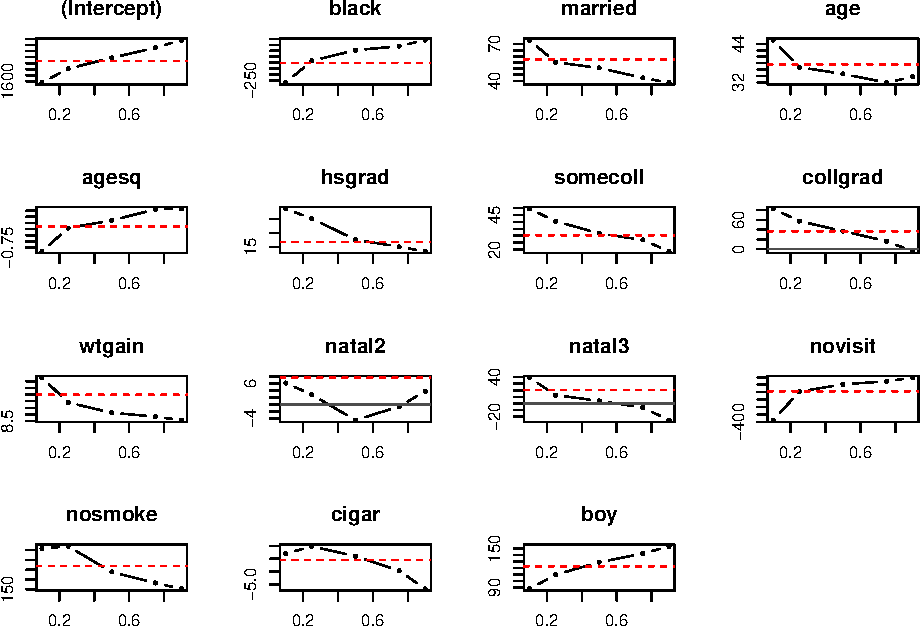
\includegraphics{Material_files/figure-latex/unnamed-chunk-26-1.pdf}

If instead we want to inspect the effect we need more points, so more
quantiles. We construct 19 observations and used the CI from the
bootstrap option (as stated on the paper). In this case we only show the
second independent variable (black dummy).

\begin{Shaded}
\begin{Highlighting}[]
\NormalTok{time_}\DecValTok{0}\NormalTok{ <-}\StringTok{ }\KeywordTok{Sys.time}\NormalTok{()}
\NormalTok{reg_exp <-}\StringTok{ }\KeywordTok{rq}\NormalTok{(formula_qr,}\DataTypeTok{tau =} \KeywordTok{seq}\NormalTok{(}\FloatTok{0.05}\NormalTok{,}\FloatTok{0.95}\NormalTok{,}\DataTypeTok{by =} \FloatTok{0.05}\NormalTok{), }\DataTypeTok{data =}\NormalTok{ data, }\DataTypeTok{method =} \StringTok{'fn'}\NormalTok{)}
\NormalTok{time_}\DecValTok{1}\NormalTok{ <-}\StringTok{ }\KeywordTok{Sys.time}\NormalTok{()}

\KeywordTok{paste0}\NormalTok{(}\StringTok{"Computing the quantiles took "}\NormalTok{,time_}\DecValTok{1}\OperatorTok{-}\NormalTok{time_}\DecValTok{0}\NormalTok{)}
\end{Highlighting}
\end{Shaded}

\begin{verbatim}
## [1] "Computing the quantiles took 30.5315752029419"
\end{verbatim}

\begin{Shaded}
\begin{Highlighting}[]
\NormalTok{sum_reg <-}\StringTok{ }\KeywordTok{summary.rqs}\NormalTok{(reg_exp, }\DataTypeTok{method =} \StringTok{'boot'}\NormalTok{)}
\end{Highlighting}
\end{Shaded}

\begin{verbatim}
## Warning in summary.rq(xi, U = U, ...): 98 non-positive fis
\end{verbatim}

\begin{Shaded}
\begin{Highlighting}[]
\NormalTok{time_}\DecValTok{2}\NormalTok{ <-}\StringTok{ }\KeywordTok{Sys.time}\NormalTok{()}

\KeywordTok{paste0}\NormalTok{(}\StringTok{"Computing the errors took "}\NormalTok{,time_}\DecValTok{2}\OperatorTok{-}\NormalTok{time_}\DecValTok{1}\NormalTok{)}
\end{Highlighting}
\end{Shaded}

\begin{verbatim}
## [1] "Computing the errors took 1.24900138378143"
\end{verbatim}

\begin{Shaded}
\begin{Highlighting}[]
\KeywordTok{plot}\NormalTok{(sum_reg, }\DataTypeTok{parm =} \KeywordTok{c}\NormalTok{(}\DecValTok{2}\NormalTok{))}
\end{Highlighting}
\end{Shaded}

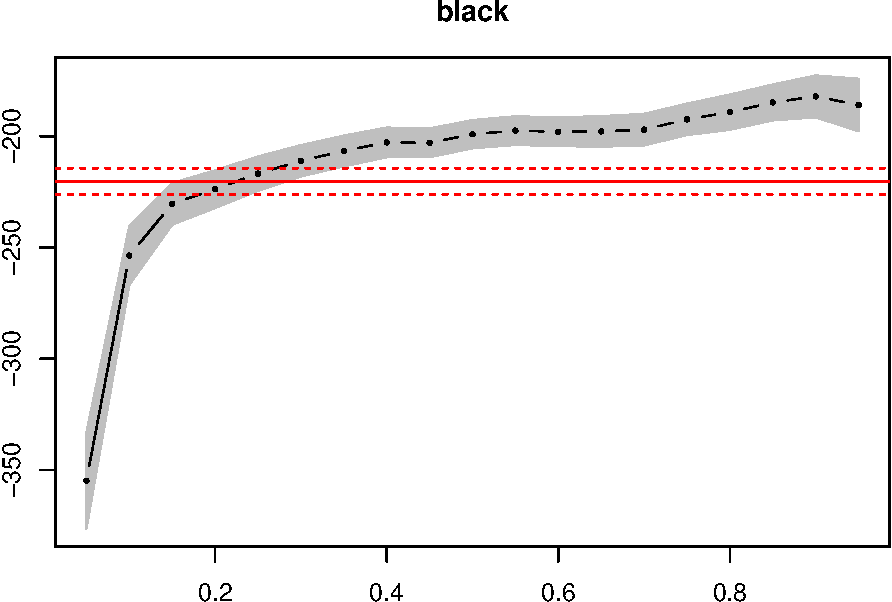
\includegraphics{Material_files/figure-latex/unnamed-chunk-27-1.pdf}

The plot shows the estimates values, the confidence intervals and the
OLS estimated value, so we can compare if the QR offers additional
insights.

\section{Exercises}\label{exercises}

\subsection{Proposed exercise 1}\label{proposed-exercise-1}

\begin{itemize}
\tightlist
\item
  Compute the quantile regression for the year 1996 to complete the
  descriptive statistics of the paper's table. Are they similar to 1992
  results? What is equal? What is different?
\item
  Compute the quantile regression for the same set of variables but for
  a recent year (after year 2000). Does the outcome change? If yes, what
  changes and how would you interpret it?
\end{itemize}

\subsection{Proposed exercise 2}\label{proposed-exercise-2}

\begin{itemize}
\tightlist
\item
  Compute the quantile regression for the year 1992 and 1996 including a
  variable of your interest. Does the result change significantly? Why
  do you consider it relevant for the analysis? How do you interpret the
  results obtained?
\end{itemize}

\section{More on quantiles}\label{more-on-quantiles}

In this section I will only list other implementations of quantile
regression that might be usefull for your future research. The list is
presentend without any particular order. If you have any suggestions,
please let me know:

\begin{itemize}
\tightlist
\item
  Decomposition methods using quantiles
  \citep{machado2005counterfactual}
\item
  Un-conditional quantiles regression \citep{firpo2009unconditional}
\item
  Decomposition methods using un-conditional quantile methods
  \citep{firpo2018decomposing}
\item
  Quantile estimation with non linear effects
\item
  Parallel quantile estimation
\item
  Quantile regression for time series (CAViaR)
\item
  Quantile regression for Spatial Data (package McSpatial)
\item
  Quantile regression for panel data, which is under development since
  it does not exist (yet) a consistent estimator (package `rqpd' and
  Ivan Canay's package)
\end{itemize}

\section{References}\label{references}

\bibliography{book.bib,packages.bib}


\end{document}
